\section{模型检验与分析}

为验证三问模型的有效性和稳健性，分别进行计算误差、硬约束和参数敏感性检验。

\subsection{数值误差与一致性核验}

问题二和问题三的收益评价经独立复核；问题三还直接比较最终经济变量的经验相关矩阵与目标矩阵。结果见表\ref{tab:error}。

\begin{longtable}{>{\centering\arraybackslash}p{0.24\textwidth}>{\centering\arraybackslash}p{0.20\textwidth}>{\centering\arraybackslash}p{0.20\textwidth}>{\centering\arraybackslash}p{0.24\textwidth}}
  \caption{模型误差与约束检查结果}\label{tab:error}\\
  \toprule
  检查项 & 问题一 & 问题二 & 问题三 \\
  \midrule
  \endfirsthead
  \caption{模型误差与约束检查结果（续）}\\
  \toprule
  检查项 & 问题一 & 问题二 & 问题三 \\
  \midrule
  \endhead
  \bottomrule
  \endfoot
  硬约束违反数 & 0 & 0 & 0 \\
  收益复算最大误差 & 独立复算一致 & $2.24\times10^{-8}$ & $4.48\times10^{-8}$ \\
  正式MIP Gap & 2.126\%，0.739\% & 小于1\% & 中档0.768\% \\
  最大相关误差 & 不适用 & 不适用 & 0.0353 \\
\end{longtable}

表\ref{tab:error}表明，三问正式方案均满足已编码硬约束，收益计算误差处于浮点舍入量级。问题三相关误差低于0.08阈值。

\subsection{灵敏度分析}

问题一改变最小面积占比，问题二改变随机种子并补充三角分布与端点情景，问题三改变关系强度并重复相关情景生成。主要结果见表\ref{tab:sensitivity}。

\begin{longtable}{>{\centering\arraybackslash}p{0.20\textwidth}>{\centering\arraybackslash}p{0.27\textwidth}>{\centering\arraybackslash}p{0.27\textwidth}>{\centering\arraybackslash}p{0.16\textwidth}}
  \caption{灵敏度分析结果}\label{tab:sensitivity}\\
  \toprule
  问题 & 参数变化 & 主要输出变化 & 判定 \\
  \midrule
  \endfirsthead
  \caption{灵敏度分析结果（续）}\\
  \toprule
  问题 & 参数变化 & 主要输出变化 & 判定 \\
  \midrule
  \endhead
  \bottomrule
  \endfoot
  问题一 & 最小面积占比0至10\% & 滞销收益变化0.726\%，半价变化0.123\% & 稳定 \\
  问题二 & 五个随机种子 & 两模式平均收益差均为正 & 有界稳定 \\
  问题二 & 三角分布与三个端点 & 无负收益，部分端点基线更高 & 条件稳定 \\
  问题三 & 强度0.15至0.55 & 收益差小于0.186\%，波动上升 & 宏观稳定 \\
  问题三 & 五个随机种子 & 相关误差0.0209至0.0460 & 稳定 \\
\end{longtable}

问题二五个种子下的配对平均收益差如图\ref{fig:q2_seed}所示，两种销售模式均保持正向。
\begin{figure}[H]
  \centering
  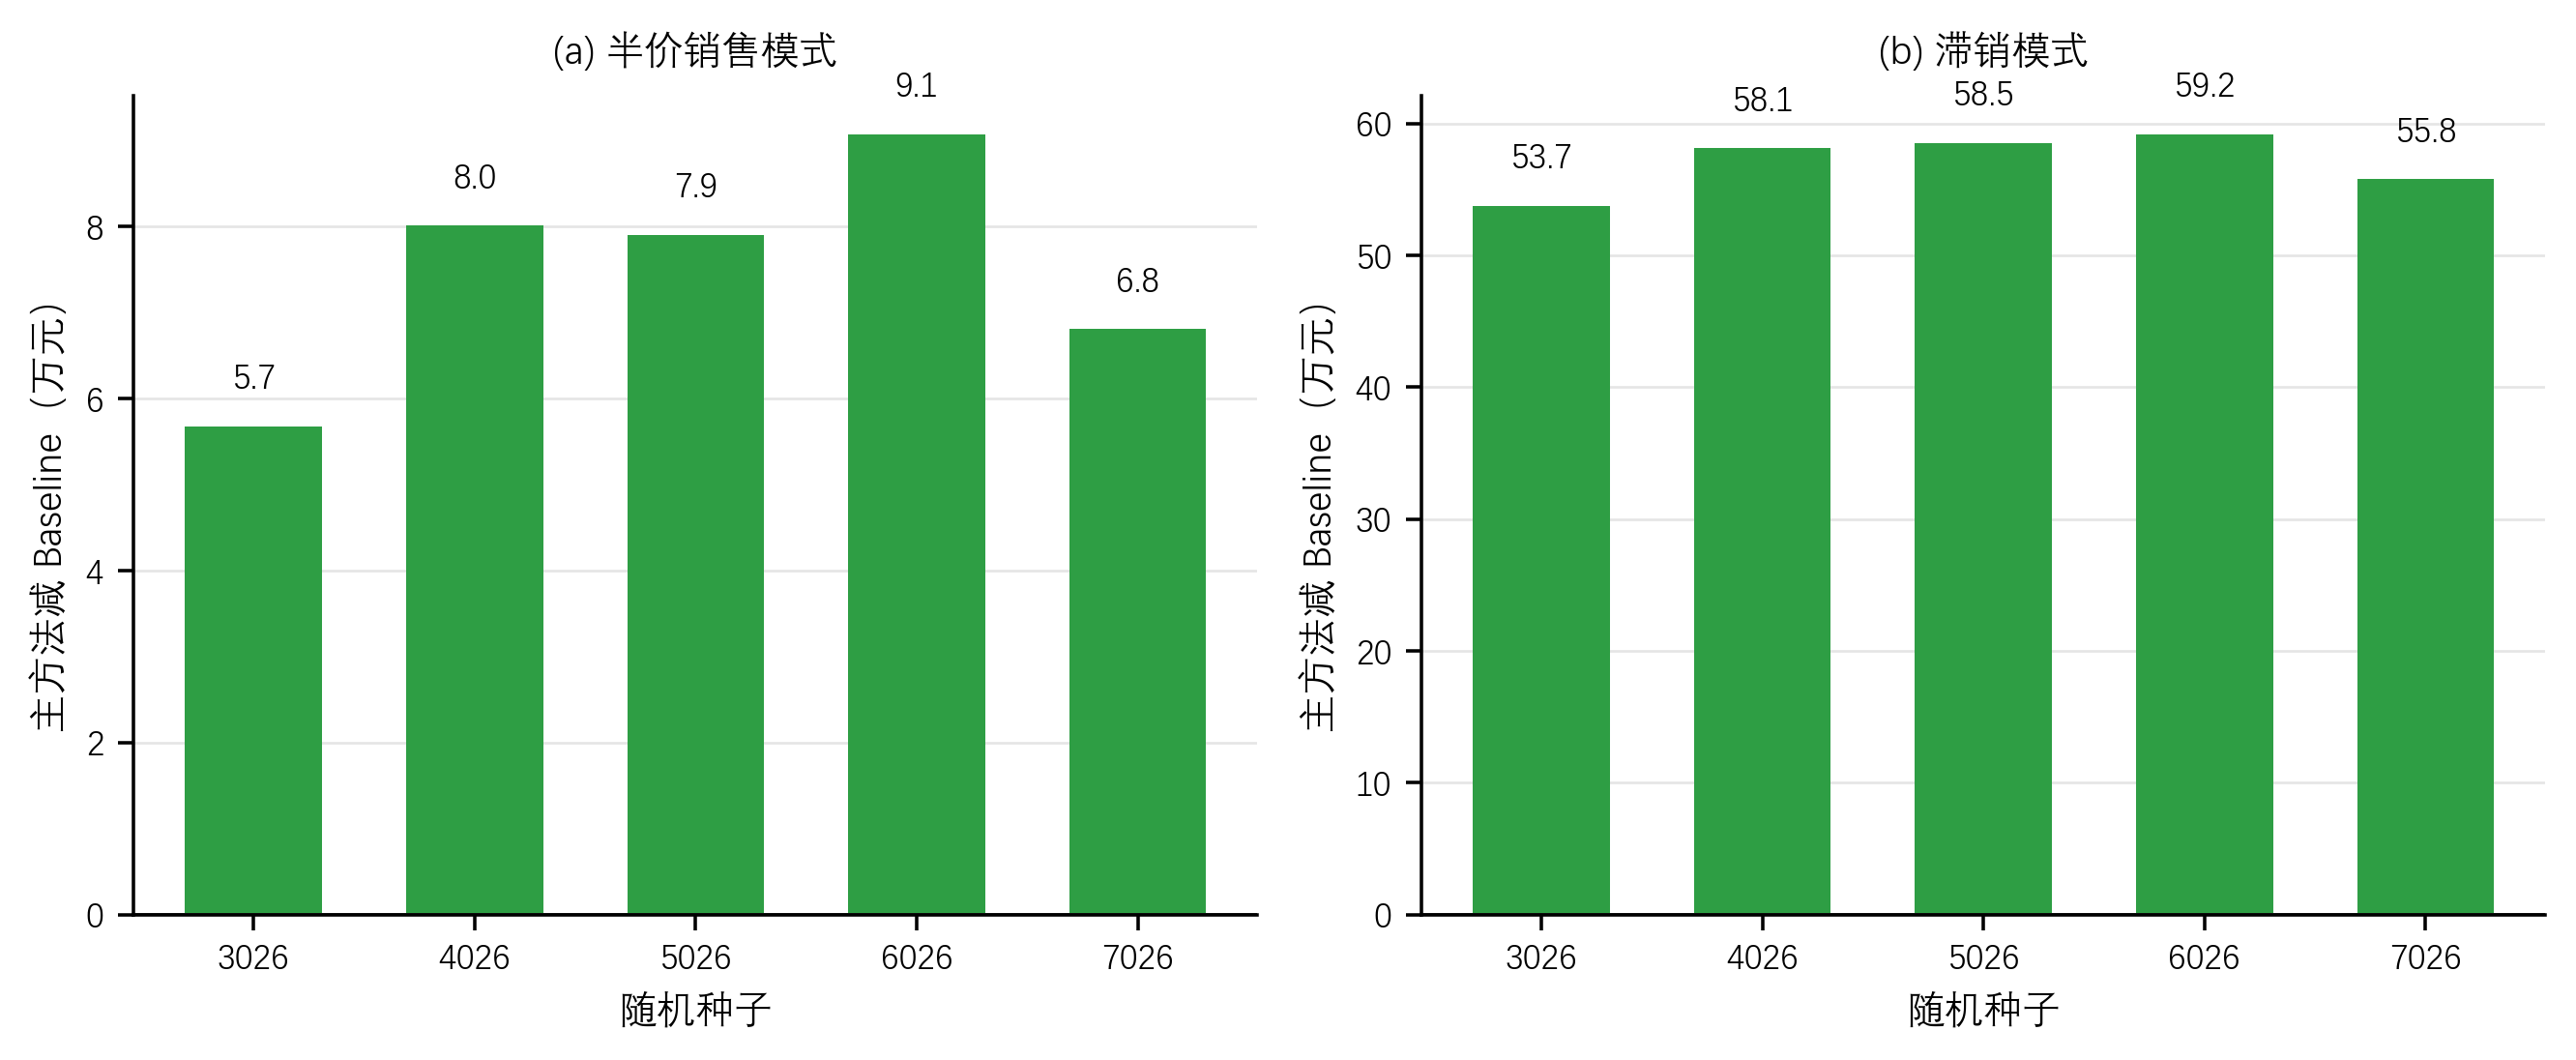
\includegraphics[width=0.92\textwidth]{figures/q2_seed_mean_profit_difference.png}
  \caption{问题二五个随机种子下的配对平均收益差}
  \label{fig:q2_seed}
\end{figure}

问题三目标矩阵与最终经验矩阵的比较见图\ref{fig:q3_corr}。所有矩阵均为正定矩阵，经验相关方向与模拟设定一致。
\begin{figure}[H]
  \centering
  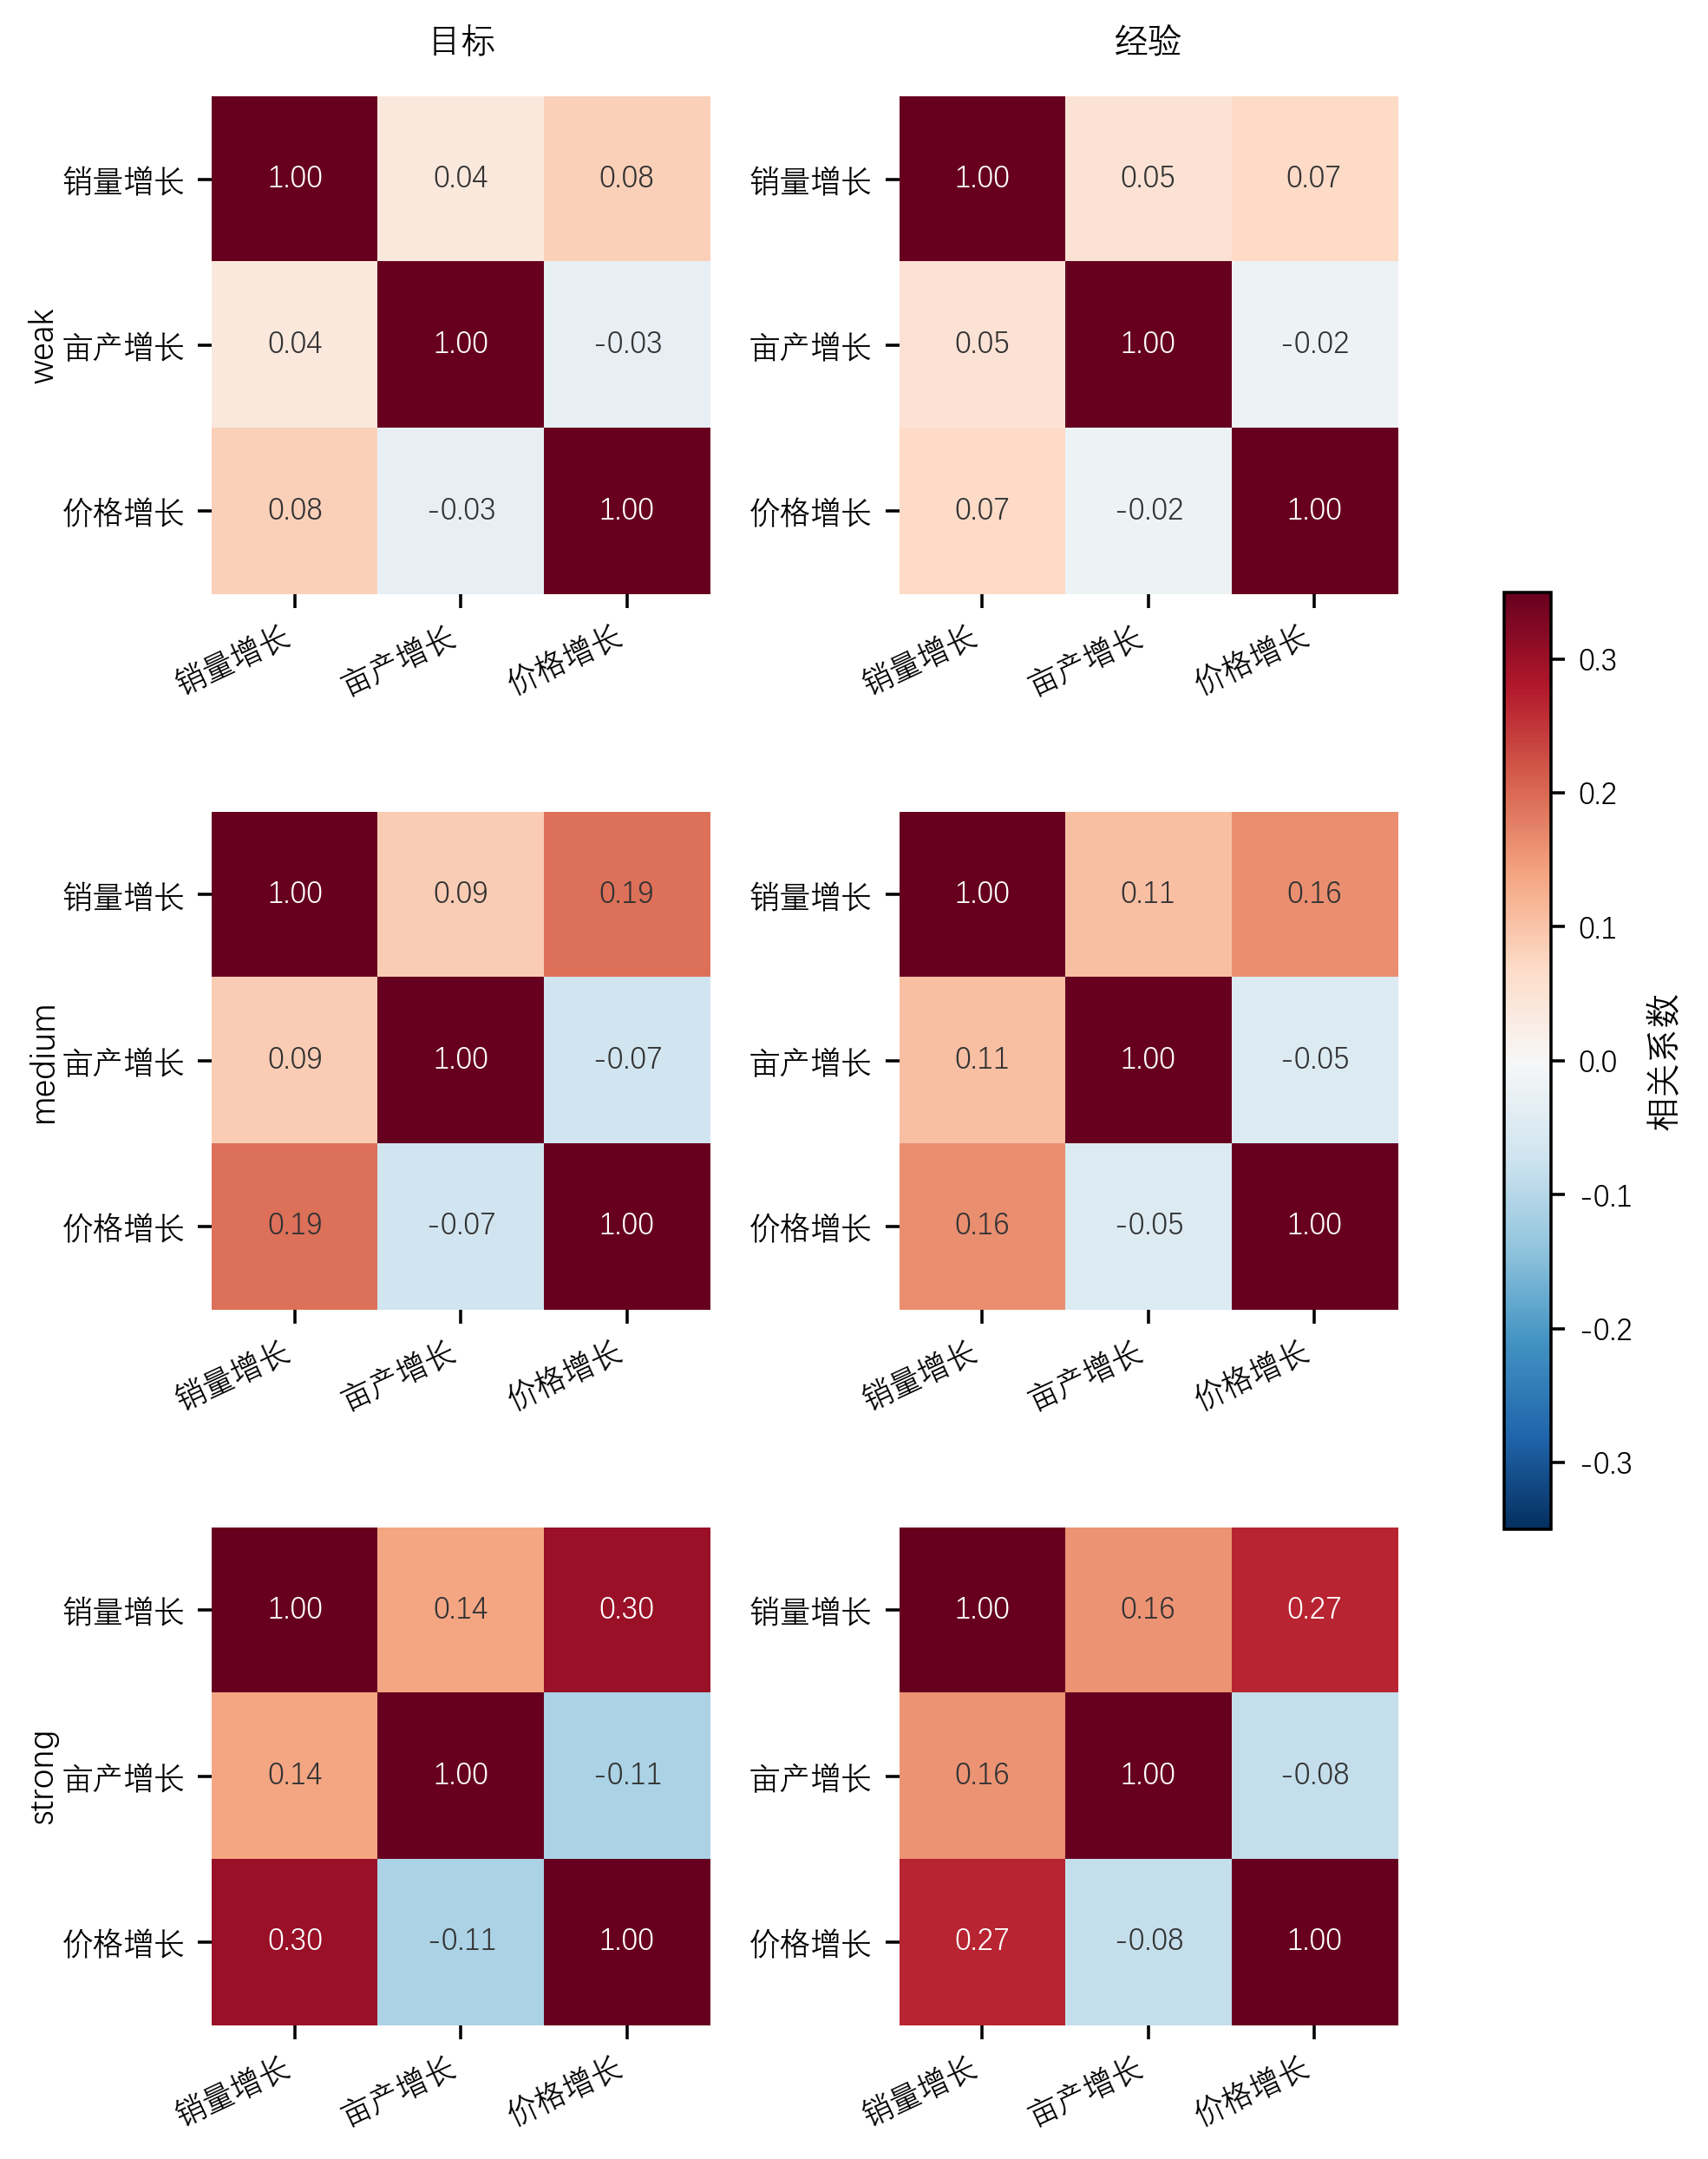
\includegraphics[width=0.76\textwidth]{figures/q3_correlation_matrix_validation.png}
  \caption{问题三目标相关矩阵与经验相关矩阵核验}
  \label{fig:q3_corr}
\end{figure}

灵敏度检验同时暴露了结论边界。问题二和问题三的半价模式下尾优势并不跨情景稳定，因此正文只陈述测试范围内无模拟亏损和跨种子平均收益方向稳定。
